\section{Dataset and Tasks}

\subsection{EuroSAT RGB}

The dataset used in this project is EuroSAT RGB. It contains 27\,000 RGB images
with a resolution of 64 x 64 pixels. Each image belongs to exactly one of ten
land-use classes. Since the RGB version was used, only the red, green, and blue
channels were available. Additional Sentinel-2 spectral bands were not used in
this project.

\begin{table}[H]
\centering
\caption{Class distribution and split used in this project.}
\label{tab:split}
\begin{tabular}{lrrrr}
\toprule
Class & Total & Train & Validation & Test \\
\midrule
AnnualCrop & 3000 & 2100 & 450 & 450 \\
Forest & 3000 & 2100 & 450 & 450 \\
HerbaceousVegetation & 3000 & 2099 & 451 & 450 \\
Highway & 2500 & 1750 & 375 & 375 \\
Industrial & 2500 & 1750 & 375 & 375 \\
Pasture & 2000 & 1400 & 300 & 300 \\
PermanentCrop & 2500 & 1750 & 375 & 375 \\
Residential & 3000 & 2100 & 450 & 450 \\
River & 2500 & 1750 & 375 & 375 \\
SeaLake & 3000 & 2100 & 450 & 450 \\
\midrule
\textbf{Total} & \textbf{27000} & \textbf{18899} & \textbf{4051} & \textbf{4050} \\
\bottomrule
\end{tabular}
\end{table}

The split was created in a stratified way with seed 42. This keeps the class
distribution in the training, validation, and test splits as similar as
possible. The small differences are caused by rounding for classes with 2500 or
3000 images.

\subsection{Binary Task}

In addition to the original 10-class task, a binary task was defined. The
classes were grouped into vegetation and non-vegetation:

\begin{table}[H]
\centering
\caption{Mapping used for binary classification.}
\label{tab:binary_mapping}
\begin{tabularx}{\textwidth}{lX}
\toprule
Binary class & EuroSAT classes \\
\midrule
Vegetation & AnnualCrop, Forest, HerbaceousVegetation, Pasture, PermanentCrop \\
Non-vegetation & Highway, Industrial, Residential, River, SeaLake \\
\bottomrule
\end{tabularx}
\end{table}

This second task is useful because it uses the same dataset but asks a different
question. It is also less fine-grained than the 10-class task. Therefore, it is
expected to be easier, because several visually similar vegetation classes are
merged into one class.

\subsection{Preprocessing}

To avoid data leakage, the split was created before any normalization
statistics were computed. The mean and standard deviation were then computed
only on the training split. The RGB statistics used were:

\begin{itemize}
  \item Mean: [0.3448, 0.3806, 0.4083]
  \item Standard deviation: [0.2031, 0.1371, 0.1156]
\end{itemize}

Training images were optionally augmented. In the final configuration this
included horizontal flips, vertical flips, and rotations up to 15 degrees. No
random augmentation was applied to validation or test images. Those images were
only converted to tensors and normalized with the training statistics.

\begin{figure}[H]
\centering
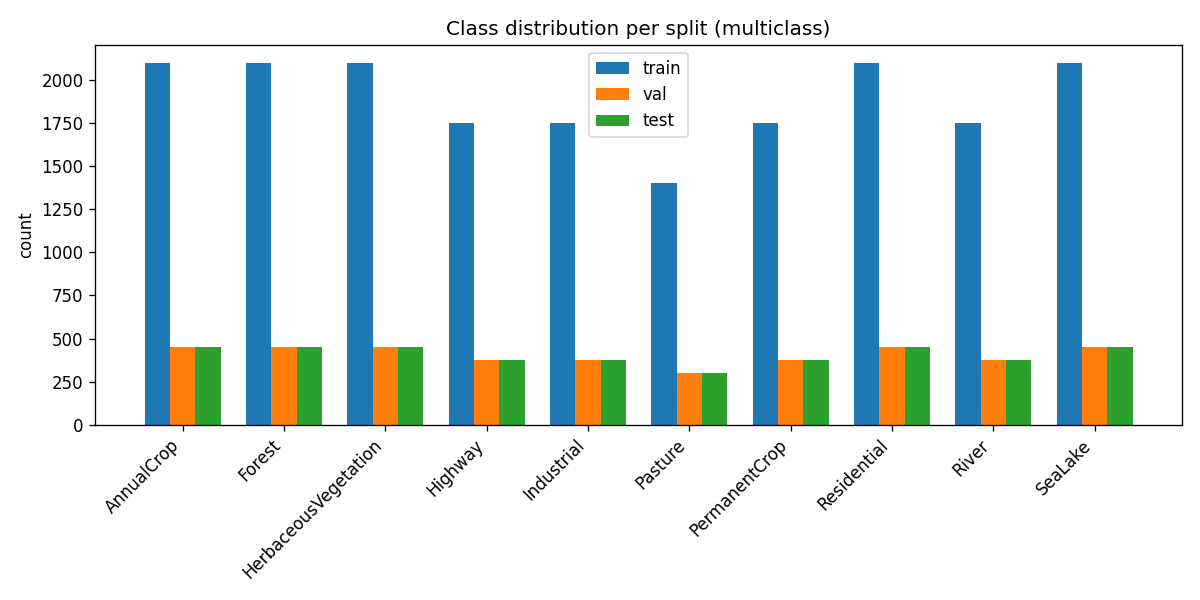
\includegraphics[width=0.85\textwidth]{../outputs/experiments/course_practical/runs/Final_multiclass/plots/class_distribution.png}
\caption{Class distribution in the final 10-class experiment.}
\label{fig:class_distribution}
\end{figure}
